\subsection{Inicialización del Bootstrap Processor: Pasaje desde modo protegido hacia modo legacy x64}
    \subsubsection{Modo Legacy x64: Modelo de segmentación}    
    La especificación multiboot nos asegura que estamos en modo protegido, pero no tenemos la certeza de tener asignada una GDT válida, es por esto que asignamos una GDT con 
    3 descriptores de nivel 0, una para datos y otras dos de código, esta diferenciación de descriptores de código es necesaria para realizar los jump far para pasar de modo real hacia modo protegido y de modo protegido-compatibilidad x64 hacia modo largo x64.

\vspace{0.5cm}
\begin{center}
    \begin{tabular}{|c|c|}
        \hline
        Indice & Descriptor\\
        \hline
        0 & Descriptor nulo\\
        \hline
        1 & Código nivel 0 para 32 bits\\
        \hline
        2 & Código nivel 0 para 64 bits\\
        \hline
        3 & Datos nivel 0 para 32 y 64 bits\\
        \hline
    \end{tabular}
\end{center}
\vspace{0.5cm}

\subsubsection{Modo Legacy x64: Modelo de paginación de los primeros 4gb}
    Se utilizó un modelo de paginación en identity mapping donde se cubren los primeros 64 GB de memoria. El modo de paginación elegido fue IA32e en 3 niveles con páginas de 2 megas, es importante remarcar que como para pasar a modo largo de 64 bits es obligatorio tener paginación activa, el mapeo de la memoria virtual fue realizado en 2 etapas, en la primera se mapearon unicamente los primeros 4gb pues desde modo protegido puedo direccionar como máximo hasta 4gb y luego desde modo largo, se completa el esquema de paginacion a 64gb agregando las entradas necesarias a las estructuras.
    \\

    Esquema de paginación IA32-e:
    \begin{itemize}

        \item \textbf{PML4: } 512 entries disponibles de 8 bytes de ancho cada una. Solo fue necesario instanciar la primera entrada de la tabla.

        \item \textbf{PDPT: } 512 entries disponibles de 8 bytes de ancho cada una. 
        Solo fue necesario instanciar las primeras 64 entradas de esta tabla.

        \item \textbf{PDT: } 32768 entries disponibles de 8 bytes de ancho cada una.
        Se instancian en modo protegido 2048 entradas para cubrir los primeros 4gb y luego desde modo largo se completan las 30720 entradas restantes completando 64 gb.
    \end{itemize}

    \begin{center}
        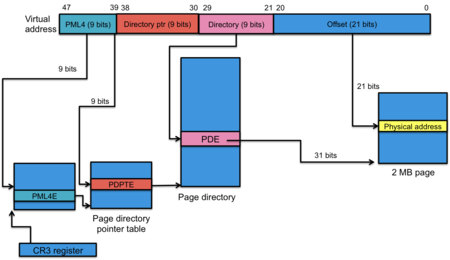
\includegraphics[height=6cm]{images/ia32e-overview-paging.png}
    \end{center}

	Luego de establecer estas estructuras, realizamos una comprobación vía $cpuid$ para saber si está disponible modo x64, de verificarse esta comprobación, encendemos los bits del procesador correspondientes para habilitar dicho modo.

    \subsection{Inicialización del Bootstrap processor: Pasaje a modo largo x64 nativo}

    Para pasar de modo compatibilidad a modo nativo de 64 bits, es necesario realizar un salto largo en la ejecucion a un descriptor de la GDT de código de 64 bits.\\
    \\
    Luego de realizar el salto al segmento de código de x64 de la GDT establecemos un contexto seguro con los registros en cero, seteamos los selectores correspondientes de la GDT y establecemos los punteros a una pila asignada al BSP.

    \subsubsection{Modo Largo x64: Extensión de paginación a 64 gb}

    En este punto ya podemos direccionar arriba de los 4gb, entonces completamos las entradas en las estructuras de paginación para completar el mapeo hasta 64gb.

    \subsubsection{Modo Largo x64: Inicialización del PIC - Captura de excepciones e interrupciones}
	
    Enviamos señales al PIC para reprogramarlo de forma tal en la que atienda las interrupciones enmascarables.
    Luego, asignamos una IDT que captura todas las excepciones e interrupciones y de ser necesario, realiza las acciones correspondientes con su ISR asociada. Particularmente las excepciones son capturadas y mostradas en pantalla y se utiliza la interrupcion de reloj para sincronizacion y esperas, las demás interrupciones son ignoradas.

    \begin{center}
        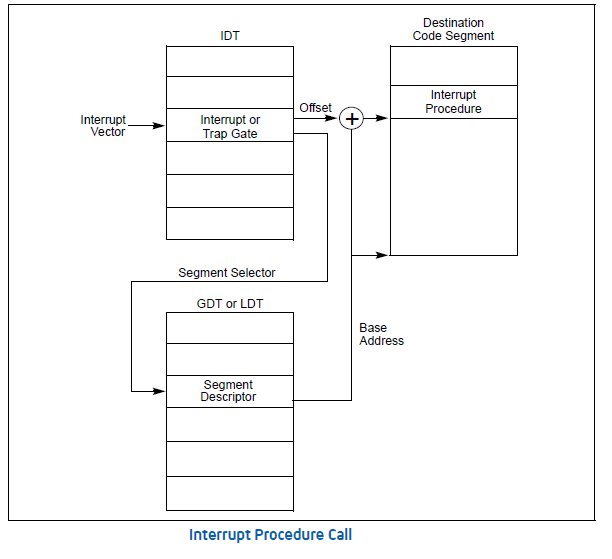
\includegraphics[height=10cm]{images/interrupts.png}
    \end{center}

\subsection{Modo Largo x64: Mapa de memoria del kernel}

\subsubsection{Estructuras de paginación en memoria}
\begin{center}
    \begin{tabular}{|c|c|}
        \hline
        Estructura & Posición en memoria\\
        \hline
        PML4T & 0x0000000000740000\\
        \hline
        PDPT & 0x0000000000841000\\
        \hline
        PDT & 0x0000000000942000\\
        \hline
    \end{tabular}
\end{center}

\subsubsection{Pilas asignadas a cada procesador}

\begin{center}
    \begin{tabular}{|c|c|}
        \hline
        Núcleo & Posición de la pila\\
        \hline
        BSP & 0x0000000000400000\\
        \hline
        AP1 & 0x0000000000500000\\
        \hline
        AP2 & 0x0000000000600000\\
        \hline
        AP3 & 0x0000000000700000\\
        \hline
        ... & ...\\
        \hline
        AP15 & 0x0000000001600000\\
        \hline
    \end{tabular}
\end{center}

\subsubsection{Variables globales y constantes del sistema}

\begin{center}
    \begin{tabular}{|c|c|}
        \hline
        Descripción & Posición en memoria\\
        \hline
        static\_variable\_area & 0x0000000000200000\\
        \hline
        start\_address & 0x0000000000200000\\
        \hline
        start\_merge\_address & 0x0000000000200001\\
        \hline
        sleep\_address & 0x0000000000200002\\
        \hline
        start\_copy\_address & 0x0000000000200003\\
        \hline
        number\_of\_cores\_address & 0x0000000000200004\\
        \hline
        seed\_address & 0x0000000000200006\\
        \hline
        array\_len\_address & 0x0000000000200010\\
        \hline
        done\_address & 0x0000000000200020\\
        \hline
        finish\_copy\_address & 0x0000000000200030\\
        \hline
        TEN\_MEGA & 0x0000000000a00000\\
        \hline
        MAX\_PROCESSOR & 8\\
        \hline
        temp\_address & 0x0000000001e00000\\
        \hline
        array\_start\_address & temp\_address + MAX\_PROCESSOR * TEN\_MEGA\\
        \hline
    \end{tabular}
\end{center}
\vspace{0.5cm}